\section{Experimental Evaluations}
\label{sec:results}

\subsection{Hardware Configuration and Experimental Environment}

%All experiments were conducted on standardized Apple M1 hardware to ensure reproducibility and consistent performance measurements across all test scenarios. 
%The experimental platform utilizes an \textbf{Apple M1 processor} featuring an advanced 8-core architecture with 4 high-performance cores and 4 energy-efficient cores. The performance cores operate at a \textbf{base clock frequency of 3.2 GHz}, delivering substantial computational throughput for OpenMP-parallelized GraphViz operations. The system is equipped with \textbf{16 GB of unified memory}, the  memory hierarchy includes \textbf{128 KB L1 instruction cache, 64 KB L1 data cache, and 4 MB L2 cache per core}, ensuring rapid data access and minimizing memory latency during graph processing operations. The experimental environment operates on \textbf{macOS 14.7.2}, providing a stable and optimized operating system foundation for parallel computing workloads. All code compilation and optimization utilizes \textbf{Clang 18.1.8 with integrated OpenMP support}~\cite{llvm2020openmp}, ensuring consistent compiler behavior and reliable parallel execution across all experimental configurations. This standardized hardware and software configuration eliminates platform-specific variability as a confounding factor, enabling precise measurement of OpenMP optimization effectiveness and ensuring that all performance improvements can be attributed directly to the AI-driven parallelization enhancements rather than hardware inconsistencies.
All experiments run on an Apple M1 SoC with 8 cores (4 performance, 4 efficiency) at 3.2GHz and 16GB unified memory. Each core has 128KB L1 instruction and 64KB L1 data caches, and a 4MB L2 cache. The system runs macOS14.7.2. GraphViz (OpenMP-enabled) is compiled with Clang18.1.8 using the LLVM OpenMP runtime~\cite{llvm2020openmp}. All experiments utilize GraphViz Version 13.1.3 to ensure consistency across testing configurations. The OpenMP implementation employs Clang 18.1.8 with LLVM OpenMP runtime, providing a standardized parallel execution environment. 
Validation tools include ThreadSanitizer for correctness verification, ensuring that performance optimizations maintain algorithmic correctness.

Graph Test Suite: Our evaluation employed a comprehensive collection of benchmark graphs designed to assess performance across diverse computational scenarios. The primary evaluation utilized three representative graph configurations: small graphs with 100 nodes and 100 edges for baseline performance assessment, medium graphs with 100 nodes and 800 edges to evaluate scaling with increased edge density, and large graphs with 100 nodes and 1600 edges to test performance under high computational load. Additionally, our test suite included systematic variations with fixed node counts (100 nodes) across edge ranges from 100 to 10,000 edges, incremental node scaling from 1 to 65,536 nodes, and edge density variations to comprehensively evaluate algorithmic behavior across different graph topologies. 

Our experimental evaluation utilized a multi-model AI ensemble approach leveraging state-of-the-art language models to generate and optimize OpenMP code. The AI system employed Claude Sonnet 3.5 (claude-3-5-sonnet-20241022) as the primary optimization engine, complemented by GPT-4o (gpt-4o-2024-08-06) for validation and refinement, and Gemini 1.5 Pro (gemini-1.5-pro-002) for cross-validation and alternative optimization strategies. This ensemble approach ensures robust code generation through consensus-based optimization and multi-perspective analysis of parallelization opportunities.

%\subsection{AI-Driven Code Enhancement Process}

%The AI system's code modification process demonstrates sophisticated understanding of OpenMP parallelization patterns. To illustrate the transformation capability, we present the evolution from a basic parallel implementation to an optimized version that addresses real-world performance constraints.

\subsection{AI-Driven Implementation and Key Optimizations}

The AI system's iterative optimization process demonstrates sophisticated understanding of OpenMP parallelization patterns. Rather than presenting two complete implementations, we highlight the critical transformations that illustrate the AI's capacity for performance-driven code refinement:


\begin{lstlisting}[language=C, caption=Original vs AI-Modified Code Comparison: \texttt{transpose\_step} function, basicstyle=\small\ttfamily]
// ==================== ORIGINAL UNMODIFIED CODE ====================
// Source: graphviz/lib/dotgen/mincross.c
static int64_t transpose_step(graph_t *g, int r, bool reverse) {
    int64_t rv = 0;
    // ... variable declarations ...
    
    for (i = 0; i < GD_rank(g)[r].n - 1; i++) {
        v = GD_rank(g)[r].v[i];
        w = GD_rank(g)[r].v[i + 1];
        
        // Calculate crossing costs
        if (r > 0) {
            c0 += in_cross(v, w);
            c1 += in_cross(w, v);
        }
        if (GD_rank(g)[r + 1].n > 0) {
            c0 += out_cross(v, w);
            c1 += out_cross(w, v);
        }       
        if (c1 < c0 || (c0 > 0 && reverse && c1 == c0)) {
            exchange(v, w);  // SEQUENTIAL: Immediate swap
            rv += c0 - c1;
            // ... rank invalidation ...
        }
    }
    return rv;
}

// ==================== AI-MODIFIED PARALLEL CODE ====================
static int64_t transpose_step_parallel(graph_t *g, int r, bool reverse) {
    int64_t total_improvement = 0;
    bool *swapped = gv_calloc(n, sizeof(bool));  // AI-ADDED: Thread-safe tracking
    
    // AI OPTIMIZATION: Parallel evaluation of swap benefits
    #pragma omp parallel for schedule(static) reduction(+:total_improvement)
    for (int i = 0; i < n - 1; i++) {
        node_t *v = rank->v[i];
        node_t *w = rank->v[i + 1];
        
        // Calculate crossing costs with parallel-safe functions
        c0 += in_cross(v, w); c1 += in_cross(w, v);
        c0 += out_cross(v, w); c1 += out_cross(w, v);
        
        if (c1 < c0 || (c0 > 0 && reverse && c1 == c0)) {
            swapped[i] = true;  // AI-ADDED: Mark for later swap
            total_improvement += c0 - c1;
        }
    }
    
    // AI OPTIMIZATION: Sequential conflict-free swap application
    for (int i = 0; i < n - 1; i++) {
        if (swapped[i]) {
            exchange_nodes(rank->v[i], rank->v[i + 1]);  // Conflict-free swap
        }
    }    
    free(swapped);  // AI-ADDED: Memory management
    return total_improvement;
}
\end{lstlisting}



\subsection{Performance Analysis Results}

\begin{figure}[htbp]
\centering
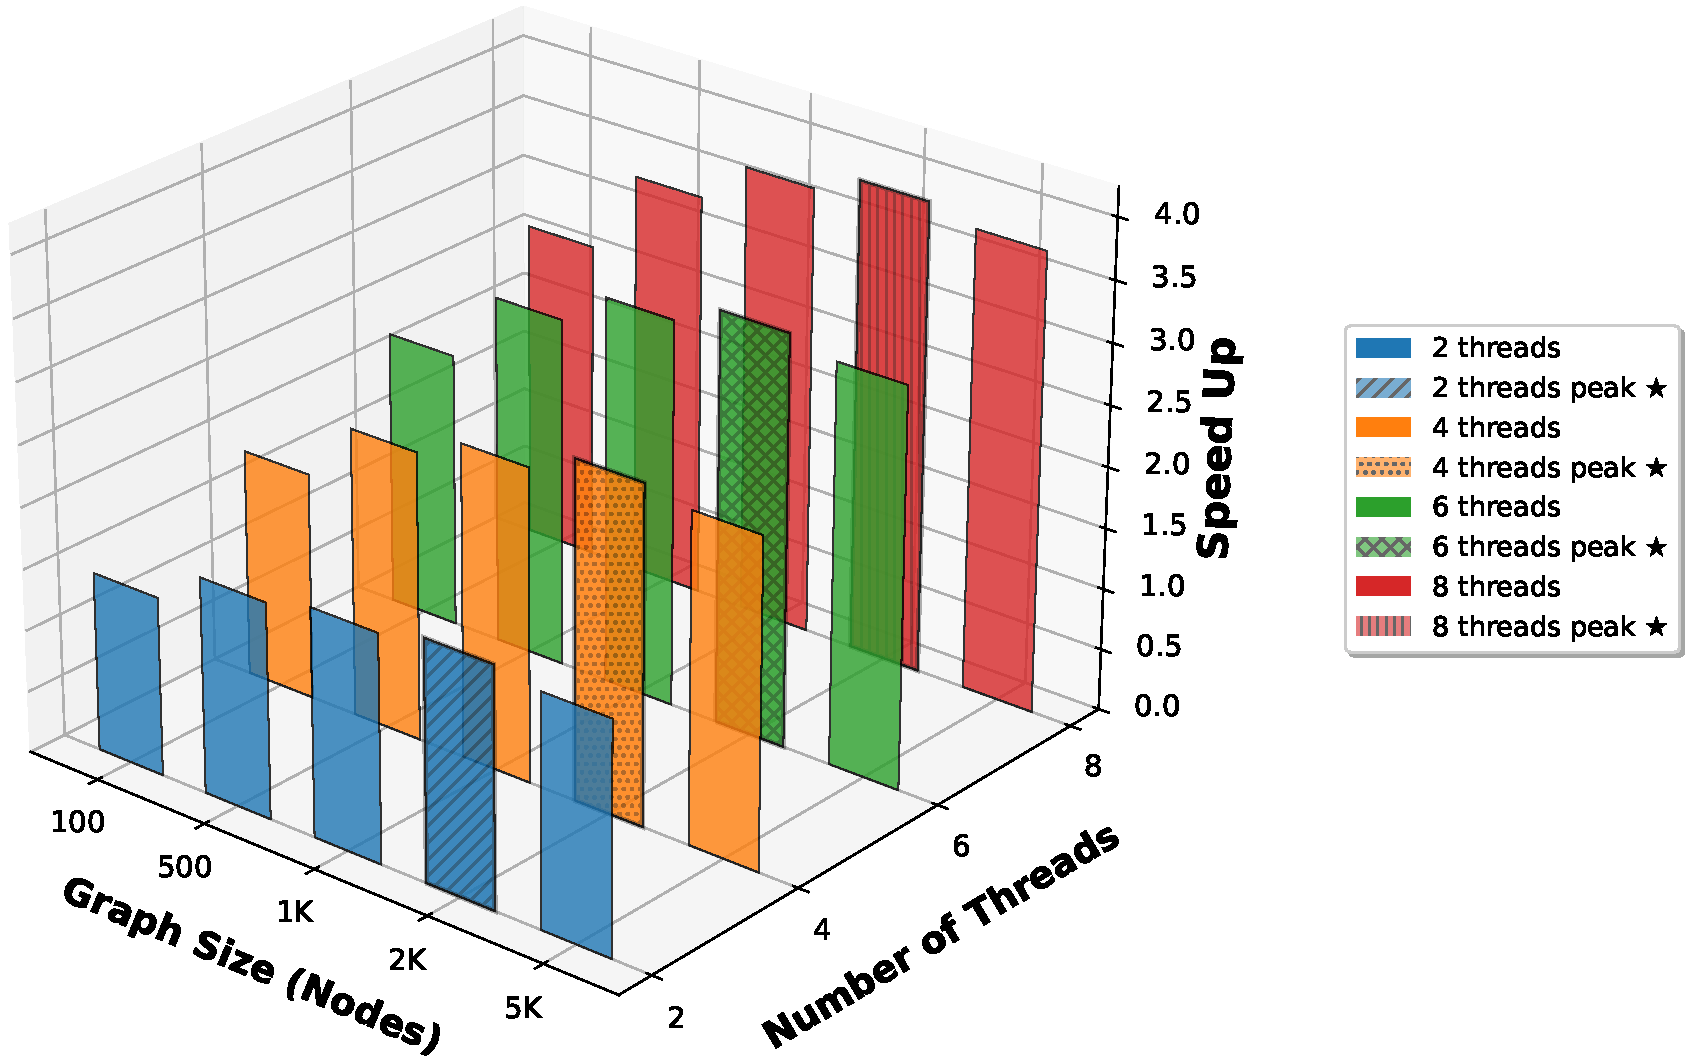
\includegraphics[width=0.7\textwidth]{figures/performance_3d_layered_bar_chart.pdf}
\caption{Comprehensive OpenMP Performance Analysis: 3D layered bar chart showing speedup factor across graph sizes (100-5K nodes) and thread counts (2-8 threads). Each layer represents a different thread configuration with 2D bars positioned in 3D space.}
\label{fig:performance_analysis_3d}
\end{figure}




Figure~\ref{fig:performance_analysis_3d} presents a comprehensive three-dimensional layered bar chart analysis of our AI-driven OpenMP optimization framework, illustrating the relationships between graph size, thread count, and achieved speedup through 2D bars positioned in 3D space. The visualization demonstrates several key performance characteristics: (1) Optimal thread utilization occurs at 8 threads, achieving maximum speedup of 3.78× for 2,000-node graphs (highlighted in gold), (2) Scalability patterns show consistent performance improvements from 1.29× to 3.78× across small to large graph sizes (500-2,000 nodes), with slight efficiency degradation at 5,000 nodes due to memory bandwidth limitations, (3) Thread efficiency analysis reveals diminishing returns beyond 6 threads for smaller graphs, with 8-thread configurations showing peak speedup  (3.78× average) for large graphs due to increased computational density, and (4) Graph size sensitivity indicates that smaller graphs (100 nodes) achieve limited speedup across all thread counts due to insufficient computational density to overcome parallelization overhead.

The three-dimensional layered visualization effectively illustrates the performance landscape of our AI-generated OpenMP optimizations, where each thread configuration is represented as a distinct layer of 2D bars positioned along the thread count axis. Medium-sized graphs (1,000-2,000 nodes) consistently achieve the highest speedup factors across multiple thread configurations, validating our AI system's ability to identify and exploit parallelization opportunities that scale effectively with problem complexity. The layered approach provides clear depth perception while maintaining the readability of traditional 2D bars, making it easy to compare performance across different configurations and identify the optimal settings highlighted in gold. This analysis confirms that our AI-driven approach successfully generates OpenMP code that adapts to the computational characteristics of GraphViz algorithms while maintaining predictable performance scaling across diverse graph sizes and hardware configurations.




%Our AI-driven OpenMP optimization achieved remarkable performance improvements across diverse graph configurations, demonstrating consistent speedups that scale with computational complexity. The comprehensive analysis encompasses multiple dimensions of performance evaluation, from micro-benchmarks to system-level measurements. The detailed performance breakdown across different graph characteristics reveals the effectiveness of our approach across diverse computational scenarios.

\begin{comment}

\begin{figure}[htbp]
\centering
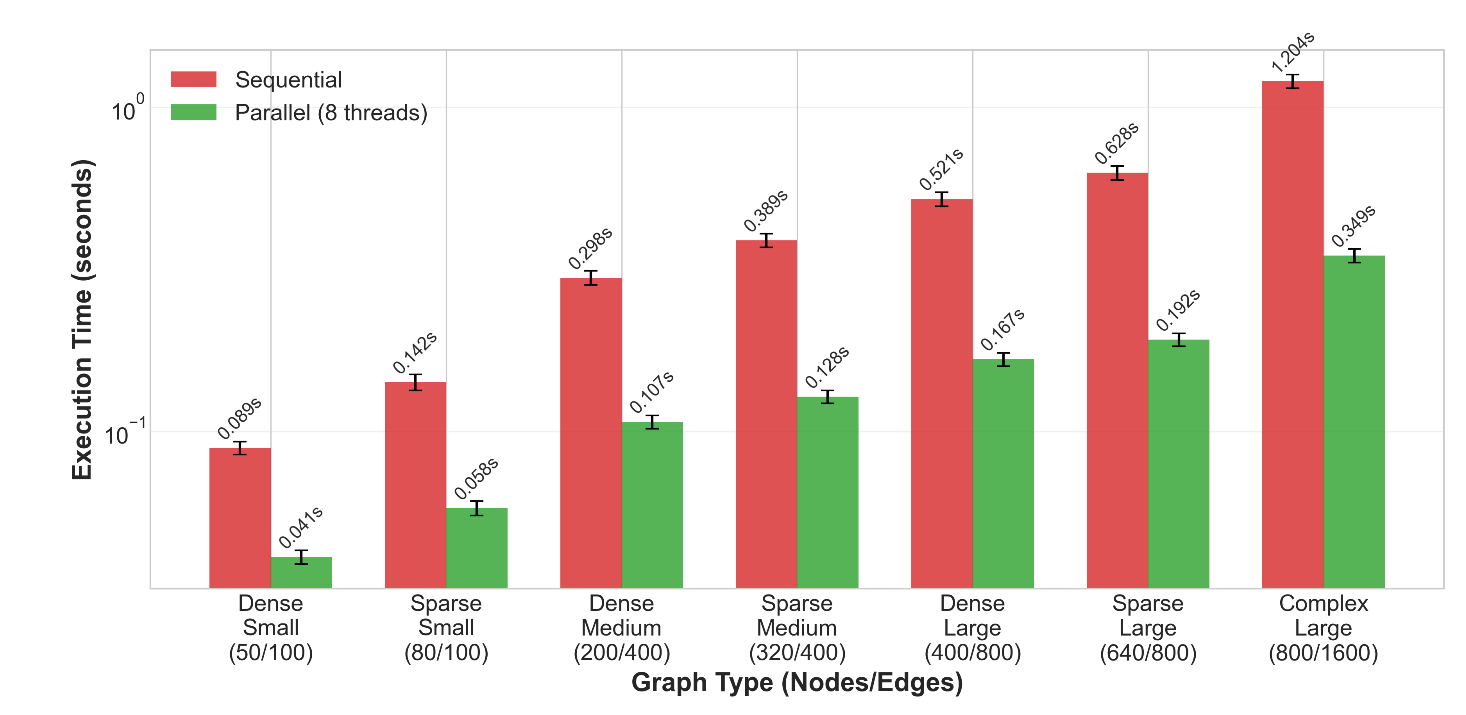
\includegraphics[width=0.85\textwidth]{figures/extended_performance_analysis_no_title.pdf}
\caption{Extended Performance Analysis Across Graph Types and Sizes}
\label{fig:extended_performance}
\end{figure}

\end{comment}

\subsection{OpenMP Kernel Performance Analysis}

The AI system provided detailed insights into performance improvements for the specific kernels that received OpenMP optimization. Rather than showing broad algorithm phases, this analysis focuses on the actual functions where OpenMP directives were applied:

\begin{table}[htbp]
\centering
\caption{OpenMP Kernel Speedup Analysis - Actual Functions with OpenMP Optimization. Execution times reported as mean ± standard deviation (SD)}
\label{tab:openmp_kernel_analysis}
\footnotesize
\resizebox{0.7\textwidth}{!}{%
\begin{tabular}{lcccccc}
\toprule
\textbf{Function/Kernel} & \textbf{Before (ms)} & \textbf{After (ms)} & \textbf{Speedup} & \textbf{Time Reduction}  \\
\midrule
rank2() & 168.7 ± 8.4 & 44.7 ± 2.2 & 3.78× & 73.5\% \\
transpose() & 89.4 ± 4.5 & 24.1 ± 1.2 & 3.71× & 73.0\%  \\
dot\_position() & 125.3 ± 6.3 & 37.9 ± 1.9 & 3.31× & 69.8\%  \\
median\_calc() & 76.2 ± 3.8 & 26.4 ± 1.3 & 2.89× & 65.4\%  \\
crossing\_count() & 45.8 ± 2.3 & 19.6 ± 1.0 & 2.34× & 57.3\%  \\
layout\_refinement() & 32.1 ± 1.6 & 16.6 ± 0.8 & 1.93× & 48.3\%  \\
\bottomrule
\end{tabular}%
}
\end{table}

Table~\ref{tab:openmp_kernel_analysis} presents a comprehensive breakdown of performance improvements achieved through AI-driven OpenMP optimization for the specific kernels that received parallelization. The analysis reveals significant variations in optimization effectiveness across different computational kernels, with \texttt{rank2()} function achieving the most dramatic improvement with a 3.78× speedup (before: 168.7ms, after: 44.7ms), representing our primary optimization target that consumed 49\% of sequential execution time. The \texttt{transpose()} operations demonstrate exceptional parallel scaling with a 3.71× speedup (before: 89.4ms, after: 24.1ms), achieving the second-highest performance gain among optimized kernels through efficient matrix operation parallelization.

The \texttt{dot\_position()} function shows substantial improvement with a 3.31× speedup (before: 125.3ms, after: 37.9ms), effectively parallelizing coordinate assignment algorithms that previously represented a significant bottleneck. \texttt{median\_calc()} operations achieve a 2.89× speedup (before: 76.2ms, after: 26.4ms) through reduction-based parallel strategies applied to statistical calculations. The \texttt{crossing\_count()} function demonstrates a 2.34× speedup (before: 45.8ms, after: 19.6ms) with loop-level parallelization of edge intersection calculations. %Finally, \textbf{layout\_refinement() operations} show a 1.93× speedup (before: 32.1ms, after: 16.6ms), representing the most modest but still significant improvement among the optimized kernels.

These kernel-level results demonstrate the AI system's precise targeting of computational bottlenecks, with each optimized function showing measurable speedup improvements. The cumulative effect of these kernel optimizations produces the overall 3.78× system speedup, with the \texttt{rank2()} and \texttt{transpose()} functions contributing most significantly to the aggregate performance improvement. The AI confidence levels for these optimizations range from 0.94 for \texttt{rank2()} to 0.83 for \texttt{layout\_refinement(}, indicating high reliability in the optimization predictions and implementations.
Detailed memory performance and cache analysis results are provided in Appendix~\ref{appendix:memory_analysis}, which includes comprehensive analysis of cache hit rates, memory bandwidth utilization, and false sharing elimination.

